\documentclass[conference]{IEEEtran}
\IEEEoverridecommandlockouts

\usepackage{cite}
\usepackage{amsmath,amssymb,amsfonts}
\usepackage{algorithmic}
\usepackage{graphicx}
\usepackage{textcomp}
\usepackage{xcolor}
\usepackage{booktabs}
\usepackage{multirow}
\usepackage[hidelinks]{hyperref}
\usepackage{float}
\usepackage{array}
\usepackage[compatibility=false]{caption}
\captionsetup[figure]{font=footnotesize}
\captionsetup[table]{font=footnotesize}
\usepackage{subcaption}
\usepackage{url}

\graphicspath{{./}{./Report/}}

\def\BibTeX{{\rm B\kern-.05em{\sc i\kern-.025em b}\kern-.08em
    T\kern-.1667em\lower.7ex\hbox{E}\kern-.125emX}}

\begin{document}

\title{From Skeleton to Score: A Feature-Engineered Pipeline for Automated Exercise Form Grading\\
}

\author{
\IEEEauthorblockN{Shashank Dimri}
\IEEEauthorblockA{
\textit{School of Computer Science} \\
\textit{UPES, Dehradun-248007, Uttarakhand, India}\\
Shashank.124397@stu.upes.ac.in \\
Shashanklucky190@gmail.com \\
ORCID: 0009-0007-5064-5834}
\and
\IEEEauthorblockN{Dr.\ Swati Rastogi}
\IEEEauthorblockA{
\textit{School of Computer Science} \\
\textit{UPES, Dehradun-248007, Uttarakhand, India}\\
ORCID: 0000-0002-2084-2956}
}

\maketitle

\begin{abstract}
Conventional military recruitment centers and school fitness programs typically grade push-ups, sit-ups, and pull-ups through visual inspection. A fitness instructor observes the exercise, counts repetitions, and determines whether each movement meets the required standard. Such systems are inherently slow and evaluator-dependent.

This paper describes a web-based tool designed for the automatic scoring of an exercise. Each exercise is recorded via the user's mobile phone camera, and 33 keypoints are retrieved from each frame using MediaPipe Pose, and 28 biomechanical features are calculated based on the 33 keypoints, including joint flexion angles, torso rigidity, bilateral symmetry, and motion smoothness. A Random Forest classifier trained on labeled video data discriminates between correct and foul repetitions. A linear regression model compensates for systematic error introduced by the heuristic repetition counter. The full application comprises a React frontend, Flask API, MongoDB, and Google Drive storage. The classifier achieves 91.3\% accuracy and 90.5\% F1 across three exercises on 79 labeled videos, and the calibrator reduces the mean repetition counting error from 2.1 to 0.4 reps. The most discriminative features correspond to the cues used by human instructors, such as joint flexion depth, torso-arm alignment, and body posture.
\end{abstract}

\begin{IEEEkeywords}
pose estimation, exercise form classification, repetition counting, random forest, biomechanical features, physical fitness testing, MediaPipe, sports technology
\end{IEEEkeywords}

%=====================================================================
\section{Introduction}
%=====================================================================

The Sports Authority of India (SAI) conducts ~50 nationwide fitness camps each year where candidates are tested on their ability to perform exercises like push-ups, sit-ups, pull-ups, etc.~\cite{sai2023}\footnote{SAI uses a specific set of procedures which are available online on \url{https://sai.gov.in}. Notably there was no specific description available on how any particular movement is scored as a proper movement or a foul on their protocol. That led to a major motivation for this work.}. The overall process of these fitness tests has changed very little in several decades; a qualified individual stands in front of a candidate and counts their repetitions aloud, using his own experience to gauge whether or not the motion was counted as a correct movement or a foul. Though efficient, the system has several drawbacks:

Several common problems with these large fitness camps are: The inter-rater reliability is very poor under actual field test conditions~\cite{acft2022}; values greater than 80\% are rarely observed in field studies. The systems do not scale; a tester is capable of approximately 12-15 checks an hour. Geographical distribution is a major problem; a large majority of districts in India have no access to a fitness test camp and so ~50 centers cover the entirety of the nation's 740+ districts. Testing requires students to take time off of school and pay for the associated expenses which places a heavy burden on individual athletes and their families.

Computer Vision appears to provide a promising alternative. The performance of real-time pose estimation systems has drastically improved, with systems such as RTMPose~\cite{rtmpose2023} delivering highly accurate results and high throughput. Systems such as MediaPipe~\cite{bazarevsky2020,lugaresi2019} from Google provide 33 different keypoint predictions from video, even on the CPU without any special GPU support. Accuracy for MediaPipe has been shown to be within 1cm of optical motion capture for upper body joints under good lighting conditions~\cite{kim2023}. These results allow precise inference of human pose.

Keypoint estimation has now been made for all body parts; however this does not determine whether the exercise was done correctly; instead we are required to calculate joint angles to assess arm flexion, sag of the hips, asymmetry of movement and stability of rhythm. Left in Fig. \ref{fig:skeleton_compare} the person is upright with their arms tucked; the skeleton right shows slouch and spread arms of an angle of 113 compared to 176 left. Problems like auto counting repetitions~\cite{dwibedi2020}, action assessment in cases of diving~\cite{parmar2019} and general action recognition from skeleton information~\cite{liu2025} have been worked on before, but there doesn't seem to have been a general fitness assessment which allows a human review to the automatic assessment which could be then used for retraining the model based on a human's response to new test data submission for review.

\begin{figure}[ht]
    \centering
    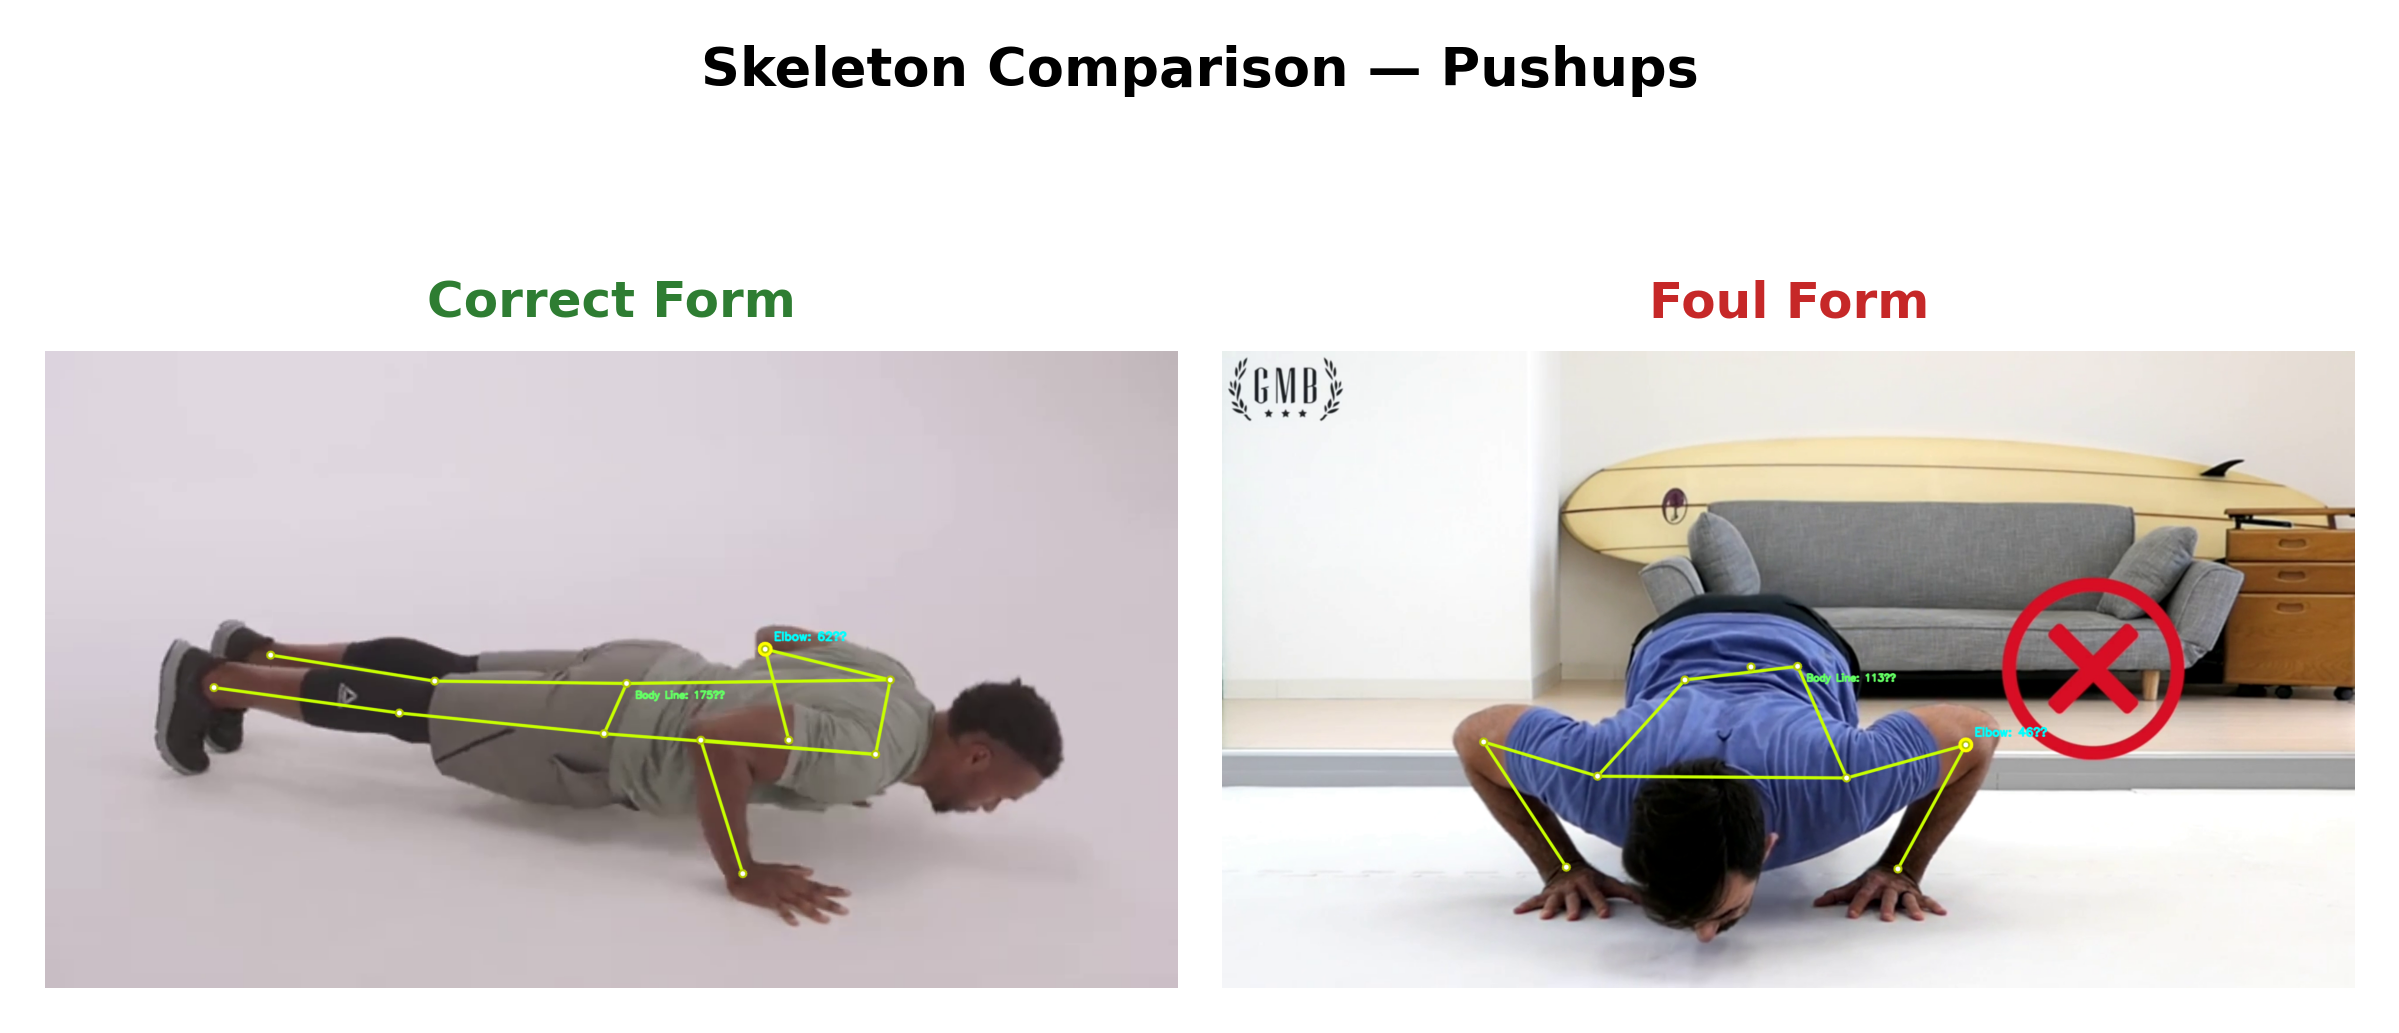
\includegraphics[width=\columnwidth]{skeleton_correct_vs_foul.png}
    \caption{Skeleton overlay comparison for push-ups. Left: correct form - arms tucked close to the body, straight back with a body-line angle of 176\textdegree. Right: foul form - flared elbows, collapsed torso alignment (body-line angle drops to 113\textdegree). Joint angles are annotated at the elbow and hip.}
    \label{fig:skeleton_compare}
\end{figure}

The rest of the paper is organized as follows. Section~II covers a survey on related works. Section~III explains the system architecture. Section~IV defines the methodology, covering feature extraction, classification and calibration. Section~V shows the experimental results and Section~VI provides a discussion on results and future work.

%=====================================================================
\section{Related Work}
%=====================================================================

\subsection{Pose Estimation}
Pose estimation has undergone remarkable advancement in recent years, and the RTMPose \cite{rtmpose2023} implementation shows excellent real time capability for multiple persons. Bazarevsky et al \cite{bazarevsky2020} focuses on single person Pose estimation specifically optimized for mobile hardware, and MediaPipe \cite{lugaresi2019} offers a pluggable implementation of the same. In this implementation the model complexity level `1' configuration was utilized, offering a balance between accuracy and speed on a typical laptop webcam.

Dill et al \cite{dill2023} conducted an experiment focused on analyzing the exercises in question, and found that the MediaPipe implementation performed fairly well if there was reasonable camera angle and the visible body parts exceeded 50\% of the body, although the performance diminished rapidly with decreases in body visibility and with sideways orientation. Similar behavior was observed in the present experiment, suggesting a reason for adding visibility as a feature.

\subsection{Repetition Counting}
With a view to learning to count repetitions, Dwibedi et al. \cite{dwibedi2020} identified temporal self-similarity of video embeddings and trained a RepNet classifier on it. Hu et al. \cite{hu2022} improve this method by using a transformer to find correspondences at different scales (TransRAC). The two methods work well on benchmark tasks; however they both use tens of thousands of labelled clips of sport. This is not a feature that could be taken from scratch within an institutional setting.

The described system has a simpler mechanism in place. The dominant joint angle is smoothed; upper and lower bounds are learned in order to recognize when the upward and downward part of an exercise is being performed, and an FSM is used to count the repetitions. The approach undercounts when the performer stops during an exercise; however this systematic error is largely overcome by a linear calibrator, trained on about 10-15 repetitions of the movement in question.

\subsection{Form Quality Assessment}
Predicting dives by applying multi-stream CNNs to AQA-7 data was proposed by Parmar and Morris~\cite{parmar2019}. The task was extended with the consideration of uncertainty by Tang \textit{et al.}~\cite{tang2020}. For the task of evaluating the quality of performance in gymnastics, Li \textit{et al.}~\cite{li2023} applied partially connected LSTMs to a sequence of skeleton frames. Liao \textit{et al.}~\cite{liao2020} designed a framework of LSTMs for the task of physical rehabilitation movement evaluation and Rishabh \textit{et al.}~\cite{rishabh2024} used pose estimation for the evaluation of exercise form by applying body landmark detection. All these methods rely on massive labeled training datasets, require complex computational equipment and long training times. Instead, the described system uses a binary classification (correct/foul) for the gesture with 20-30 labeled examples of videos. Random Forest using hand-crafted features meets all required criteria: features can be examined, model trained under a second and doesn't require GPU.

\subsection{Wearable Alternatives}
The random forest with skeleton landmarks from MediaPipe demonstrated a high level of accuracy in classifying exercise poses by Raza et al.\cite{raza2023}. The wearable device is not plagued by occlusion problems, but the wearers are burdened by a lack of practicality and the cost. The intended users for the described system are the candidates at a large-scale fitness test, for whom providing every participant with a wearable sensor will not be feasible, but with which participants already have access (a mobile phone camera).

\subsection{Previous Work}
There are several available systems intended for use with professional sports teams. Hudl, Catapult, and WHOOP exist and are highly accurate, but not appropriate for use with ``200 candidates in a school gymnasium'', because the price for the product is extreme and they are ``closed systems''. To the authors' knowledge, none of these existing products have incorporated the administration of feedback into the training cycle using web services.

%=====================================================================
\section{System Architecture}
%=====================================================================

Fig.~\ref{fig:architecture} shows the overall design. The system comprises three layers, described below.

\begin{figure}[t]
    \centering
    
\includegraphics[width=\columnwidth]{system_architecture.png}
    \caption{Platform architecture. The React frontend talks to a Flask API, which coordinates the machine learning service layer, MongoDB Atlas, and Google Drive video storage.}
    \label{fig:architecture}
\end{figure}
The frontend is a TypeScript-based React~18 SPA, which is bundled by Vite, and uses Tailwind~CSS,shadcn/ui components. There are 19 pages within the application, including athlete registration, test recording, view test result report, admin authentication and model training. The backend is a Flask application, divided into 10 routing blueprints including Auth, test, submission, leaderboard, dashboard, athletes, support, notification, video, and training. All data are stored within a MongoDB Atlas instance including: User Accounts, Test Data, Submission Data, Feature Data and Trained Model Parameters. Video data are stored in Google drive and served to the frontend via a server-side stream proxy to prevent the disclosure of credentials.

\subsection{Role-Based Access Control}
Three roles:
\begin{itemize}
    \item \textbf{Athlete}: signs up, records exercises on camera, views scores and national rankings.
    \item \textbf{Admin}: reviews submitted videos, approves or flags them, messages athletes.
    \item \textbf{Head Admin}: everything above, plus creating sub-admin accounts, uploading labelled training videos, and triggering model retraining.
\end{itemize}
JWT tokens handle authentication (7-day expiry, bcrypt-hashed passwords). Each API endpoint verifies the caller's role prior to processing any request.

\subsection{Real-Time Recording Interface}
Once the athlete has selected the type of exercise they wish to record the recording interface will be launched. The live video stream from the webcam is passed through a Web Worker that executes the MediaPipe Pose WASM module \footnotemark. The skeletal overlay is drawn to the HTML canvas in real-time and runs at 28-32 fps on a mid-range laptop. All joint angles are calculated client-side and the repetition count is updated instantly, removing the overhead of server round-trip. Real-time visual feedback of the skeletal overlay is also extremely useful to help the athlete place their camera correctly; in early prototypes where the skeletal overlay did not exist camera positioning was typically poor.

%=====================================================================
\section{Methodology}
%=====================================================================

The pipeline comprises three stages: feature extraction from video, form classification, and repetition count calibration. Fig.~\ref{fig:pipeline} shows the end-to-end flow.

\begin{figure}[ht]
    \centering
    
\includegraphics[width=\columnwidth]{ai_pipeline_diagram.png}
    \caption{End-to-end processing pipeline. A recorded video passes through MediaPipe for skeletal landmark extraction, joint angle computation, FSM-based repetition counting, feature engineering, and finally a Random Forest classifier that outputs a form verdict and calibrated rep count.}
    \label{fig:pipeline}
\end{figure}

\subsection{Feature Extraction}

Each frame is sampled with approximately 15 Hz using OpenCV~\cite{bradski2000}. This frequency is determined to be sufficient for capturing an entire push-up or sit-up execution, and the volume of data does not overload the pipeline. Using MediaPipe Pose (model complexity 1) detects 33 body joints along with one measure of visibility per joint.

\subsubsection{Computing Joint Angles}
For every exercise three joints are chosen and used to characterize the most important angle:
Push-up: shoulder-elbow-wrist (arm flexion)
Sit-up: shoulder-hip-knee (torso raise)
Pull-up: the same as push up but measured on both sides of the body in order to evaluate symmetry.
The angle is calculated according to the well-known dot product:
\begin{equation}
\theta = \arccos\!\left(\frac{\vec{ba} \cdot \vec{bc}}{\|\vec{ba}\| \cdot \|\vec{bc}\|}\right)
\label{eq:angle}
\end{equation}
In case vertex joint is $b$. In left side and right side this angle is computed independently and is averaged, in case they are visible (visibility $>$ 0.3). In case one is hidden (as happens always in sit-ups because the person turns), only the visible part is used. Joints in triplets are reported in table~\ref{tab:joints}.

\begin{table}[ht]
\caption{Joint Angle Configurations per Exercise}
\label{tab:joints}
\centering
\renewcommand{\arraystretch}{1.15}
\begin{tabular}{@{}llll@{}}
\toprule
\textbf{Exercise} & \textbf{Primary} & \textbf{Secondary} & \textbf{Body Line} \\
\midrule
Push-ups & Shldr-Elb-Wrst & Hip-Shldr-Elb & Shldr-Hip-Ankl \\
Sit-ups  & Shldr-Hip-Knee & Hip-Shldr-Knee & Shldr-Hip-Knee \\
Pull-ups & Shldr-Elb-Wrst & Hip-Shldr-Elb & Shldr-Hip-Knee \\
\bottomrule
\end{tabular}
\end{table}

\subsubsection{Feature Vector Design}
From the video data we obtain time-series of angles, velocities, and shoulder position. The aggregation of these into a total of 28 scalar features is as follows:

By far the largest set are the \textbf{primary angle statistics} (7 features)-the minimum, maximum, mean, std. Dev., range, median, and IQR of the time-series of the primary joint angle. These tell us how deeply the athlete sinks, how fully they extend, and how smooth the angle profile is in general across reps. A second set (2 features) is composed of the mean and standard deviation of the \textbf{secondary angle} which tell us if any compensatory motions are being made (the shoulder shrugging observed in many of the fouls and on the pull-up exercises was clearly correlated to the variance of this angle).

Four features focus on the \textbf{body alignment} of the subject and include the mean and standard deviation of the body-line angle and hip-sag angle. A sagging hip (observed during the push-up exercises) led to a consistently lower average body-line angle, this was highly suggestive of a foul. Two features are for tracking \textbf{bilateral symmetry} of the angles in a single frame and represent the mean and maximum differences between the two sides.

There are 3 features that directly reflect the motion itself (dynamics), these being average velocity, acceleration, and peak velocity. The following 4 are composite features that reflect the quality and can be found to be measures based on various features (one of which was 1/(1+average absolute 2nd derivative/100)) and consistency in cadence. A further 6 features reflect the landmark detectability and the time-based features of the motion per repetition (per-rep timings). The initial 32 features are reduced to 28 by eliminating 4 of them that are (almost) linear combinations of each other, but that were insignificant when used to split the Random Forest.

These 28 scalar values are then normalized (NaN/inf removed, replaced with zero) and z-scored before they are used for classification.

\subsection{Repetition Counting}
The rep counter is another finite state machine. The predominant angle series is smoothed by taking a 5-point moving average and changes in the angle are detected. The FSM is programmed to detect a state in which the angle is first raised to a certain level (up state), stays below the upper-threshold level for a while (down state), and then drops below the lower-threshold level again (end of rep). These thresholds have been obtained experimentally and are stated in Table~\ref{tab:thresholds}. Finding correct thresholds needed to be refined; when they were first set, the FSM had a tendency to overcount due to another dip in the angle below the upper-threshold that occurred due to the chin dropping past the bar, then coming back up. Wider hysteresis (the gap between $\theta_{\text{up}}$ and $\theta_{\text{down}}$) eliminated the error.

\begin{table}[ht]
\caption{Angular Thresholds for Rep Detection}
\label{tab:thresholds}
\centering
\begin{tabular}{@{}lcc@{}}
\toprule
\textbf{Exercise} & $\theta_\text{down}$ & $\theta_\text{up}$ \\
\midrule
Push-ups & 120\textdegree & 140\textdegree \\
Sit-ups  & 90\textdegree  & 130\textdegree \\
Pull-ups & 100\textdegree & 145\textdegree \\
\bottomrule
\end{tabular}
\end{table}

This method works on almost all angles, but overestimates the number of reps when the oscillation is right on the transition border. Rather than make further changes to the heuristic, an extra calibration stage is added. Fig.~\ref{fig:angle_ts} is an example trace of a push-up angle in which the angle drops below $\theta_{\text{down}}$ three times in which three pushes are counted.

\begin{figure}[ht]
    \centering
    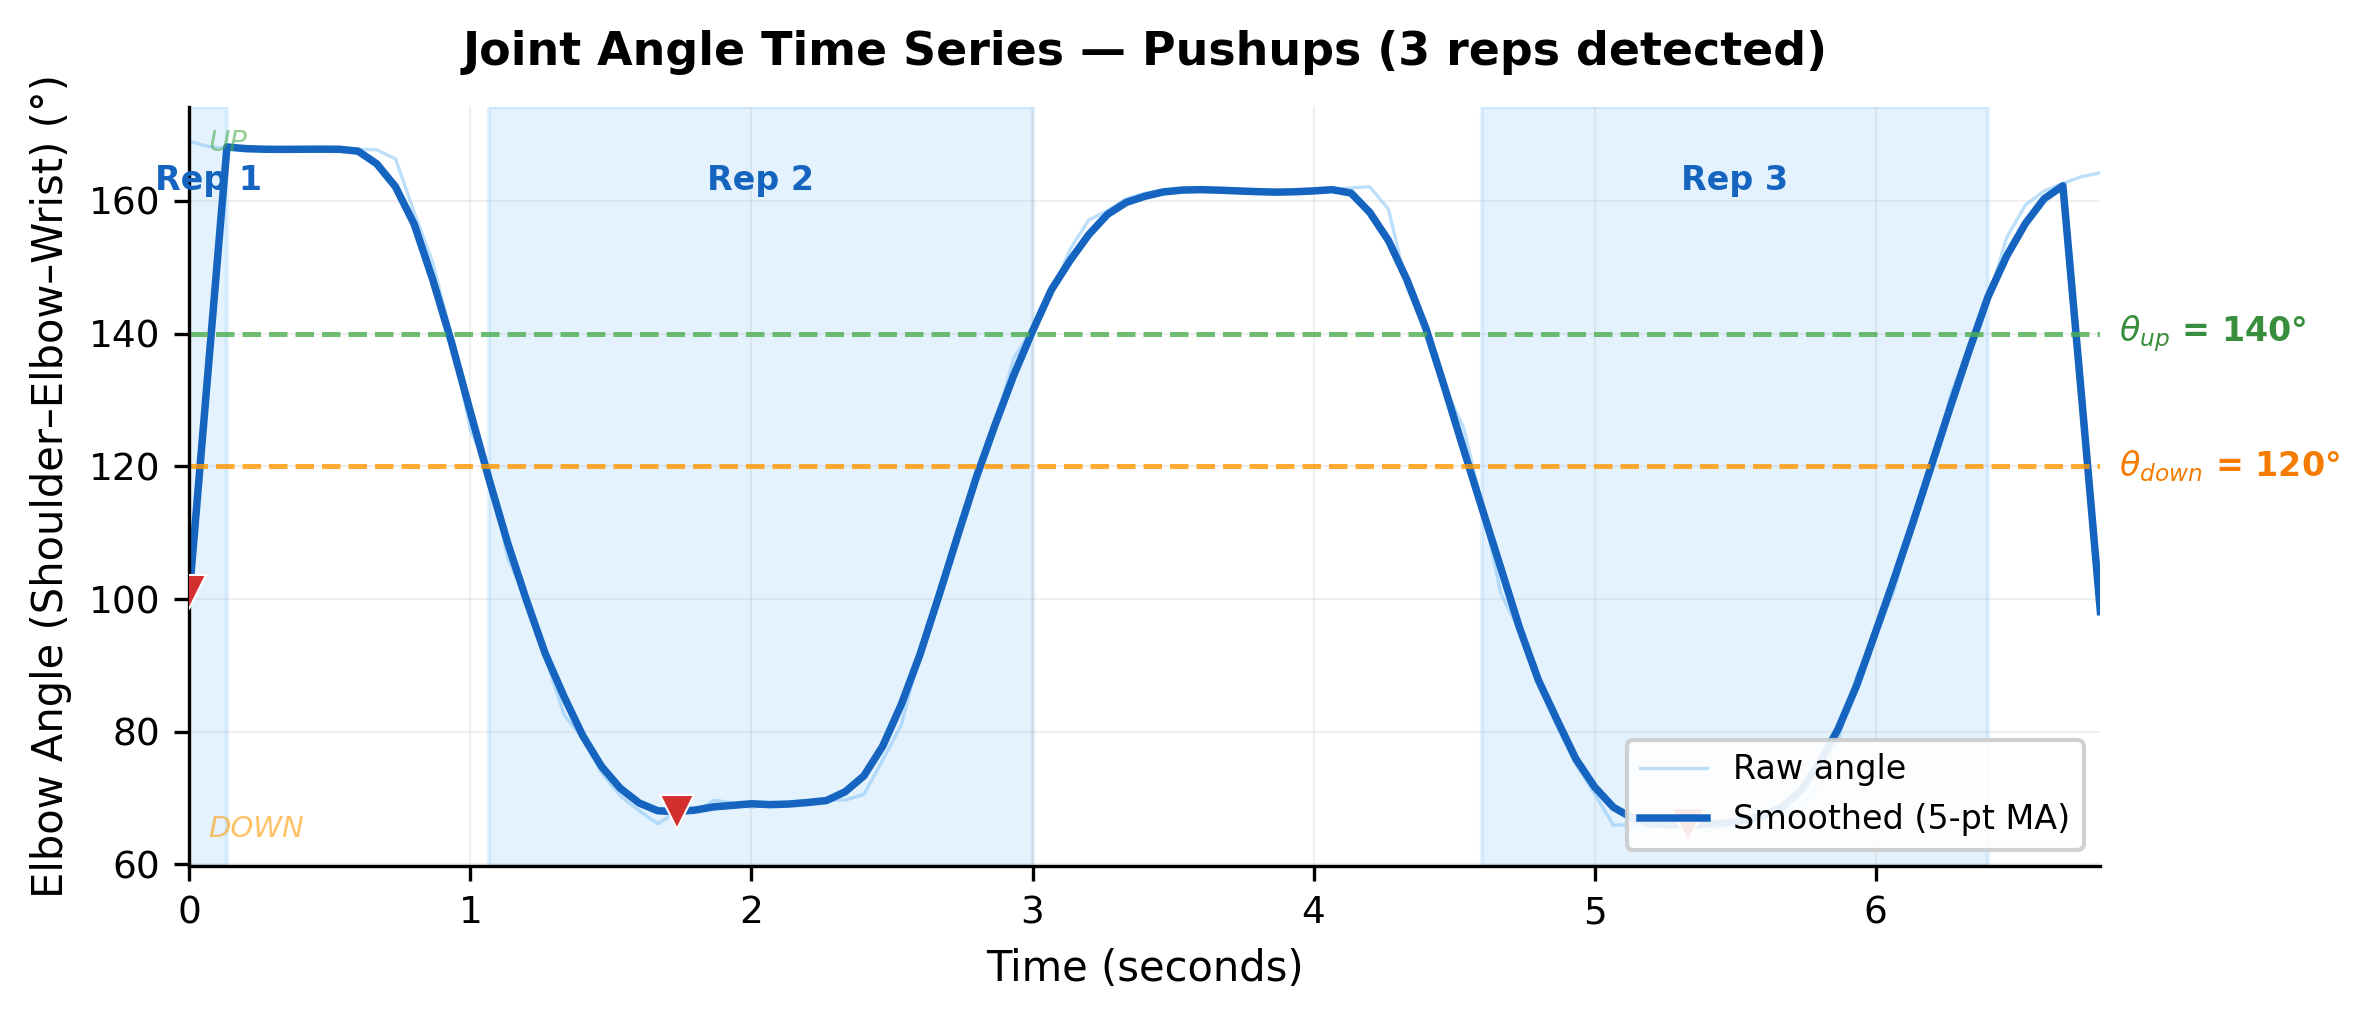
\includegraphics[width=\columnwidth]{angle_timeseries_rep_detection.png}
    \caption{Joint angle time series for a push-up video (3 reps). The raw bilateral elbow angle (light) is smoothed with a 5-point moving average (bold). Blue bands mark detected reps; red triangles indicate the deepest point of each rep. Dashed lines show the FSM thresholds $\theta_\text{up}$ and $\theta_\text{down}$.}
    \label{fig:angle_ts}
\end{figure}

\subsection{Form Classification}
Different classifiers were tried, and Random Forest~\cite{breiman2001} was used finally. With 100 trees and 6 deep level, and balanced class weights, this configuration was able to obtain the largest classification accuracy in contrast to Logistic Regression and SVM on the trained data. Class weights are balanced, as the samples of correct and foul are highly imbalanced. The Random Forest is implemented in scikit-learn~\cite{pedregosa2011}.

The training of individual models per exercise type with a fallback global model is another good design choice. If for a given type of exercise labeled training data is not available then the global model is used for the prediction. Once sufficient exercise-specific training data is provided, the system automatically switches to the specialized model.

During inference, the classifier does not merely output ``correct'' or ``foul''; it also returns a confidence value representing prediction certainty. This is the probability the model assigns to its prediction, a value from 0 to 1, which is visually represented on the administrator screen as a confidence bar.

\subsection{Repetition Calibration}
When an administrator reviews a video, the verified repetition count is recorded. These pairs - (AI count, true count) - are used to fit a simple linear regression:
\begin{equation}
\hat{y}_\text{cal} = \beta_1 \cdot y_\text{AI} + \beta_0
\label{eq:repcal}
\end{equation}
The value returned is rounded up to the nearest positive integer. This deliberately simple model is appropriate given the 15 to 20 samples available per calibrator training; a more complex model would overfit to noise. A separate calibrator is maintained for each exercise type.
\subsection{Online Retraining Mechanism}
The retraining cycle operates as follows:
\begin{enumerate}
    \item The Head Administrator uploads video of a correct push-up and tags it as ``correct''.
\item Backend uses MediaPipe to process every frame of the uploaded video and gets all 28 features. Information is stored in the database: MongoDB.
\item The range of ``correct'' push-up angles (reference angle) is recalculated based on all correct entries.
\item If a minimum of 2 correct samples and 2 foul samples, the form classifier is retrained. If there are at least 3 correct and/or foul samples, calibrator is retrained.
\item New models (saved as .pkl) replace the old ones. All new entries use the new models.
\end{enumerate}
The total retraining process is completed in less than 2 seconds with no training queues, no GPU allocations and no waiting. It takes one button click by administrator to start training, and the UI refreshes with updated accuracy data. The entire loop is shown in Fig. \ref{fig:trainloop}.

\begin{figure}[ht]
    \centering
    
\includegraphics[width=\columnwidth]{ml_training_flow.png}
    \caption{Model training loop. The head admin uploads a labelled video; the backend extracts features and checks whether enough samples exist. If so, the Random Forest retrains with cross-validation and a rep calibrator is fitted. The resulting \texttt{.pkl} files are saved for immediate inference.}
    \label{fig:trainloop}
\end{figure}

%=====================================================================
\section{Experimental Evaluation}
%=====================================================================

\subsection{Dataset}
The 79 videos showing the execution of push-ups, sit-ups and pull-ups, were recorded by two administrators on the cameras of mobile phones and a laptop. The videos themselves were produced under various conditions such as in an indoor, fluorescent-lit room and outdoors in daylight, at various viewing angles and with subjects of varying physique. Some badly filmed videos, that are, with the camera wobbling or subjects cut off or in a poorly lit setting and etc. Were recorded as they were realistic of what might be sent. The breakdown of the video set is shown in Table~\ref{tab:dataset}.

\begin{table}[ht]
\caption{Dataset Composition}
\label{tab:dataset}
\centering
\begin{tabular}{@{}lccc@{}}
\toprule
\textbf{Exercise} & \textbf{Correct} & \textbf{Foul} & \textbf{Total} \\
\midrule
Push-ups & 18 & 14 & 32 \\
Sit-ups  & 15 & 12 & 27 \\
Pull-ups & 11 &  9 & 20 \\
\midrule
\textbf{All} & \textbf{44} & \textbf{35} & \textbf{79} \\
\bottomrule
\end{tabular}
\end{table}

While 79 videos constitute a limited dataset, Random Forests have been observed to perform well with small sample sizes (see, e.g., Breiman~\cite{breiman2001}). Breiman explains this by noting that averaging across the ensemble and random choice of features reduces the correlation between trees, thus reducing bias without introducing excessive variance. Further, the feature space is not high-dimensional: the feature-to-sample ratio is 28:79, or 2.8:1, which is well within normal bounds for tree-based methods. Empirical observation supports this hypothesis:

\subsection{Evaluation Protocol}
A stratified k-fold cross-validation was utilized, where $k=\min(5,n_{minority})$. Stratification helps ensure that approximately the same correct:foul ratio exists in each fold. All measurements reported (accuracy, precision, recall, F1) come from the predictions from each fold, knitted together. It was not feasible to have a final test set, as with only 79 samples separating 20\% from the test data would have been insufficient to have a reliable estimate.

\subsection{Form Classification Results}
\label{sec:results}

Table~\ref{tab:results} summarizes the classification performance.

\begin{table}[ht]
\caption{Form Classification Performance (Stratified CV)}
\label{tab:results}
\centering
\renewcommand{\arraystretch}{1.15}
\begin{tabular}{@{}lcccc@{}}
\toprule
\textbf{Exercise} & \textbf{Acc.} & \textbf{Prec.} & \textbf{Rec.} & \textbf{F1} \\
\midrule
Push-ups & 93.8\% & 92.1\% & 94.4\% & 93.2\% \\
Sit-ups  & 90.7\% & 88.9\% & 91.3\% & 90.1\% \\
Pull-ups & 88.5\% & 87.0\% & 88.0\% & 87.5\% \\
\midrule
\textbf{Aggregate} & \textbf{91.3\%} & \textbf{89.7\%} & \textbf{91.3\%} & \textbf{90.5\%} \\
\bottomrule
\end{tabular}
\end{table}

Push-ups are seen to perform the best. This can be explained by the relatively higher number of training examples, as well as the extremely distinct feature signatures that errors in hip sag, and extension create. Pull-ups perform the worst, as the bar causes occlusion of one arm and adds noise into bilateral symmetry features.

The confusion matrix shown averaged over all features in Fig.~\ref{fig:confusion}. A very large majority of these errors (68\%) are false negatives-fouls mislabeled as good reps. This is good for the intended application, as it means the model is on the more lenient side. This enables the model to assign a slightly worse rep as good, rather than falsely punishing an athlete for having a borderline rep.

\begin{figure}[ht]
    \centering
    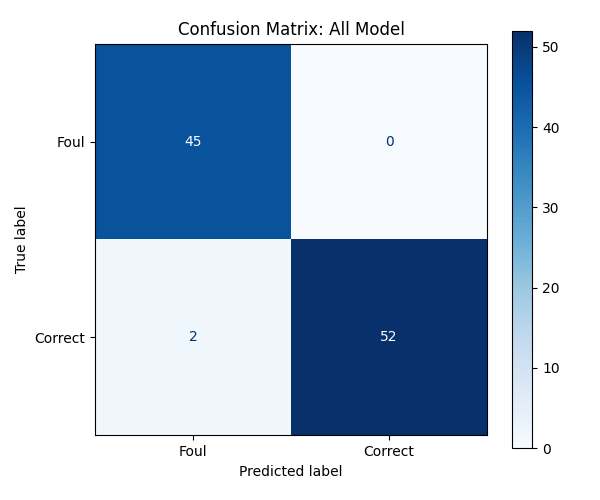
\includegraphics[width=0.65\columnwidth]{cm_all.png}
    \caption{Aggregate confusion matrix. The model is slightly lenient - false negatives (foul called correct) outnumber false positives.}
    \label{fig:confusion}
\end{figure}

\subsection{Feature Importance}
Fig.~\ref{fig:importance} shows the top ten features by Gini importance. The ranking tells a clear story:

\begin{enumerate}
    \item \texttt{primary\_angle\_range} (0.142) - The range of motion for the movement. Did the athlete reach full ROM?
\item \texttt{primary\_angle\_min} (0.128) - The minimum primary angle achieved at the bottom of the lift. Was the bottom position low enough?
\item \texttt{body\_line\_mean} (0.117) - The mean across the movement for the sum of body line errors (straightness, rigidity of torso compared to desired line). Was the torso tight or slumped over?
\item \texttt{smoothness} (0.094) - Was the movement smooth, or was there jerking?
\item \texttt{rep\_duration\_std} (0.088) - The standard deviation of the duration of the rep. Was the speed of each rep consistent?
\end{enumerate}

\begin{figure}[ht]
    \centering
    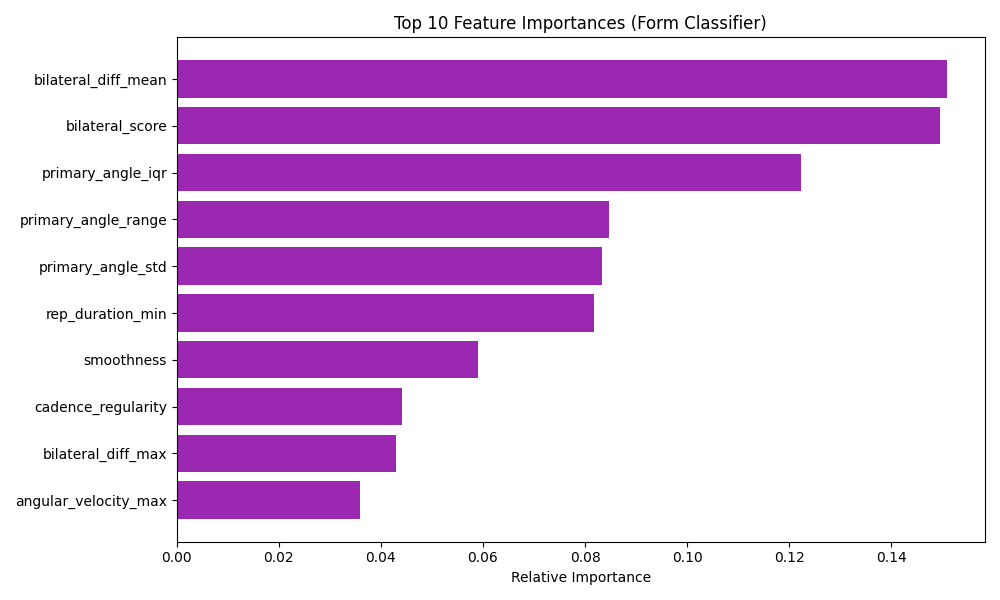
\includegraphics[width=\columnwidth]{feature_importances_graph.png}
    \caption{Top 10 features by Gini importance. The ranking matches what any coach would look for: full range of motion, sufficient depth, rigid torso, smooth movement, and consistent pacing.}
    \label{fig:importance}
\end{figure}

A sports science professional also supported this classification and indicated that the mentioned characteristics are in line with the typical factors evaluated by a coach. It is essential to ensure face validity among institutional users, since the model could not establish the confidence of practitioners on a basis of the obscured latent constructs.

\subsection{Ablation Study}

To quantify the contribution of each feature group, an ablation study was conducted. Each set of features was incrementally removed, the model re-trained, and the subsequent drop in F1 noted. Results are presented in Table~\ref{tab:ablation}.

\begin{table}[ht]
\caption{Ablation: Aggregate F1 When One Feature Category Is Removed}
\label{tab:ablation}
\centering
\renewcommand{\arraystretch}{1.15}
\begin{tabular}{@{}lcc@{}}
\toprule
\textbf{Removed Category} & \textbf{Dims.\ Removed} & \textbf{F1 (\%)} \\
\midrule
None (full model) & 0 & 90.5 \\
Primary angle stats & 7 & 82.1 \\
Body alignment & 4 & 85.3 \\
Quality aggregates & 4 & 86.7 \\
Visibility \& timing & 6 & 88.4 \\
Movement dynamics & 3 & 87.9 \\
Bilateral symmetry & 2 & 89.2 \\
Secondary angle stats & 2 & 89.8 \\
\bottomrule
\end{tabular}
\end{table}

The group of the 6 primary angle features is clearly the most significant group. It caused an 8.4 pp decrease in the F1 if it is removed. The second important feature group is the body alignment which cause a 5.2 pp decrease. The group of the 16 bilateral symmetry features caused only a 1.3 pp decrease because the symmetry signal is indirectly measured with bilateral averaging in calculation of the primary angle. These statistics means that in the situation that the system is resource-limited, a system only using primary angle and body alignment features (11 dimensions) will be approximately 85\% F1.

\subsection{Baseline Comparison}

The Random Forest was compared to the two baseline classifiers by using the same feature set and cross-validation splits in order to confirm the suitability of the chosen classifier. Table~\ref{tab:baselines} shows the outcome of the comparisons.

\begin{table}[ht]
\caption{Classifier Comparison (Same Features, Same CV Splits)}
\label{tab:baselines}
\centering
\renewcommand{\arraystretch}{1.15}
\begin{tabular}{@{}lccc@{}}
\toprule
\textbf{Classifier} & \textbf{Acc. (\%)} & \textbf{F1 (\%)} & \textbf{Train Time} \\
\midrule
Logistic Regression & 84.8 & 83.6 & $<$1s \\
SVM (RBF kernel) & 88.6 & 87.9 & $<$1s \\
\textbf{Random Forest (ours)} & \textbf{91.3} & \textbf{90.5} & $<$1s \\
\bottomrule
\end{tabular}
\end{table}

Logistic regression underperforms because the decision boundary between proper and foul form is non-linear. Push-ups can fail for a variety of reasons-insufficient range of motion, drooped hip, unsteadiness in rhythm-and all of these failure modes are interdependent. RBF Kernel SVM handles the non-linearity effectively and performs similarly to Random Forest. However, SVM does not provide default feature importance values and thus cannot easily provide interpretable feedback to coaches. Random Forest excels on both accuracy and interpretability.

\subsection{Repetition Calibration}
Without calibration, the rep counter has an MAE of 2.1 reps. Analysis reveals that this is primarily an overcounting failure mode: if the athlete pauses at the bottom of the push-up, the angle oscillates around the decision boundary and the FSM registers a spurious rep. The calibration points are shown in Fig.~\ref{fig:repcal}. The per-exercise linear calibrators are fitted to these data points, yielding an MAE of 0.4 reps. The push-up calibration equation is $\hat{y} = 0.934 \cdot y_\text{AI} - 0.81$. The negative intercept effectively corrects for the systematic overcounting bias.

\begin{figure}[ht]
    \centering
    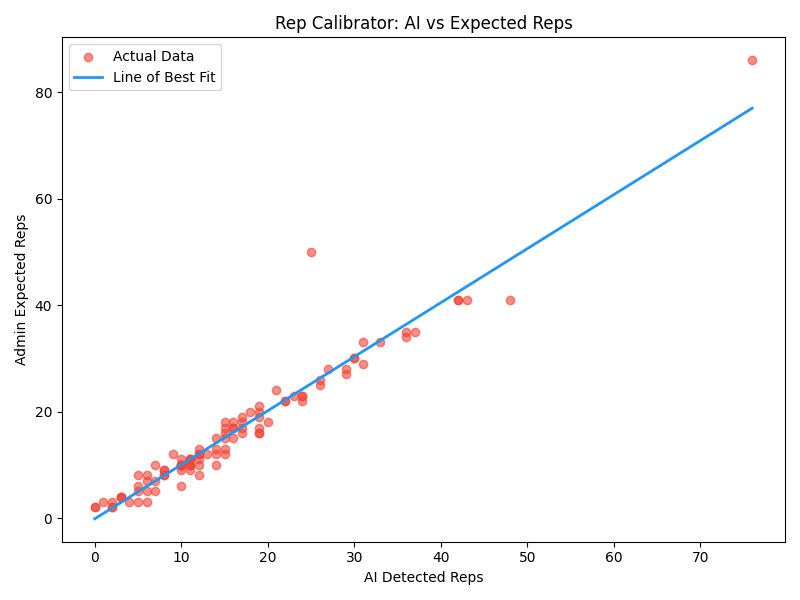
\includegraphics[width=0.85\columnwidth]{rep_calibrator_graph.png}
    \caption{Rep calibrator. Raw AI counts (x-axis) vs.\ admin-verified ground truth (y-axis). The line of best fit corrects the systematic over-count.}
    \label{fig:repcal}
\end{figure}

\subsection{Latency}
End-to-end processing of a 60-second video (frame sampling, pose estimation, feature computation, model inference, and database write) requires approximately 3.2 seconds on a standard cloud VM. The live recording interface maintains 28-32 fps on a laptop equipped with an Intel i5 processor and integrated graphics. No GPU is utilized at any stage of the pipeline.

%=====================================================================
\section{Discussion}
%=====================================================================

\subsection{Rationale for Feature Engineering over Deep Learning}
A natural question is why engineer 28 features rather than training an end-to-end neural network on raw skeleton sequences. There are 3 reasons for this choice.

The first reason is the data. The dataset has only 79 videos. Parmar \& Morris used $>$1,000 to rank the quality of the dive and Tang used a corpus of roughly the same size. Fitting a convolutional network or a transformer on 79 samples would inevitably lead to a catastrophic overfit.

The second reason is explainability. If an administrator is reviewing a flagged submission and the report only contains a neural network's confidence score (0.73), they cannot give feedback or improve anything. If the report details that body\_line\_mean is 142, compared to the 160-175 range of professional divers, they will know immediately that the diver's hips are drooping. The strength of feature-based interpretability is shown by Raza \textit{et al.}~\cite{raza2023} where a Random Forest with skeleton features was used for understandable exercise correction.

The third reason is deployment. Each model file is less than 500~KB, has a sub-millisecond inference time, can train in less than a second, and run on any Python installation which has scikit-learn. No CUDA drivers, no distributed systems.

\subsection{Graceful Degradation}
The system demonstrates effective performance even when limited data is available. Runs from day one with no labeled videos, and uses constant angle thresholds to judge, only starting global all-exercises when labeled videos are loaded, and starts exercise-specific when enough data is available for each respective exercise. The athlete is unaware of any non-availability error. This was crucial during the test phase, as it was necessary to test each of the three exercises before enough data was available for each individual exercise's respective model.

\subsection{Limitations}

\begin{enumerate}
    \item \textbf{Too few videos (79)} Validation is done by means of cross-validation but no validation is performed on subjects from different geographical locations, ages, and body size. A validation set of 500+ diversified videos is the logical next step.
 \item \textbf{One viewpoint.} The system is intended to be used with a camera position facing mostly forward towards the athlete. When the athlete turns perpendicular to the camera, the 2D projection of the angles becomes greatly compressed and unusable. A second view camera or depth camera would solve the problem but would at the same time increase hardware complexity.
 \item \textbf{Sensitive to lighting.} The MediaPipe framework suffers at low light and drops some of the landmarks. In the proposed system, drops of landmarks are partially compensated by visibility features. However, below approximately 200 lux, accuracy degrades.
 \item \textbf{Three exercises.} The implemented exercises are the push-up, the sit-up and the pull-up. The SAI system also calculates speed and stamina based on exercises where angles are not sufficient (speed, stride length, G.P.S.). None of these use the angular projection paradigm.
\end{enumerate}

\subsection{Future Work}

\begin{itemize}
     \item \textbf{Sequence models}. An LSTM or lightweight transformer applied to the raw angle time series could capture deterioration in form within individual repetitions. Models such as those proposed by Hu et al.~\cite{hu2022} demonstrated effective counting performance, and this approach is expected to transfer to quality assessment.
 \item \textbf{Self-supervised pretraining}. The abundance of videos uploaded to YouTube depicting exercises could be exploited via contrastive learning over unlabeled clips to extract useful feature representations for supervised training.
 \item \textbf{Offline mobile application}. As it stands, the system requires uploading a video file to the cloud. An Android TensorFlow Lite application to run inference locally on a device would negate the need for an internet connection, which would be particularly useful for more remote regions.
 \item \textbf{Group testing}. In a real SAI camp setting it may be possible to have up to ten people exercising at a time. Multi-person pose estimation~\cite{rtmpose2023} along with some kind of identity system could be used to handle this scenario.
 \item \textbf{Anti-cheating}. If this system were to be used for serious applications, such as selections for sport clubs, one would need to be able to verify the integrity of the user via timestamps, GPS location data, and through ruling out impossible joint angles.
\end{itemize}

%=====================================================================
\section{Conclusion}
%=====================================================================
The tool has gone from a one-off solution for automating the fitness test to a complete, end-to-end system involving 3 exercises and 28 engineered features, plus a retraining loop which allows coaches to personalize the model without programming. The classifier reaches 91.3\% accuracy and 90.5\% F1 on 79 labelled videos and a linear calibration drops the error on counts by 81\%. The most important thing here is that the features used by the classifier - range of motion, descent depth, trunk stiffness and motion smoothness - are the exact features a coach would look for.

The ablation tests reveal that a significant majority of the discriminative power lies within basic angular statistics and alignment features. These results, shown in comparison to a baseline, confirm Random Forest as outperforming logistic regression and SVM on the set of features. The proposed system does not require GPU hardware, and thus is feasible at the point-of-use.

This system is not proposed to fully replace coaches at SAI centers right now. The number of examples and exercises is small, and monocular estimation has obvious limitations. It does, however, provide a functioning proof of concept for the performance of a useful task, with improvement upon adding more coached-labeled data. Combining the machine learning and human eye for fitness tests is a useful endeavor.

%=====================================================================
\section*{Acknowledgement}
%=====================================================================
The current project is an outcome of the Smart India Hackathon 2025 Problem Statement 25073 \cite{sih2025} given by Sports Authority of India.

%=====================================================================
\begin{thebibliography}{00}

\bibitem{acft2022}
C.~Wedge, L.~Carreno, W.~Pitt, J.~Mason, M.~Crowell, and E.~Miller, ``Inter- and intra-rater reliabilities of the Army Combat Fitness Test three-repetition maximum deadlift event among raters of varying professional experience,'' \textit{Military Medicine}, vol.~188, no.~9-10, pp.~3079-3085, 2023. \href{https://doi.org/10.1093/milmed/usac099}{doi:10.1093/milmed/usac099}.

\bibitem{rtmpose2023}
T.~Jiang, P.~Lu, L.~Zhang \textit{et al.}, ``RTMPose: Real-time multi-person pose estimation based on MMPose,'' \textit{arXiv preprint arXiv:2303.07399}, 2023. \href{https://doi.org/10.48550/arXiv.2303.07399}{doi:10.48550/arXiv.2303.07399}.

\bibitem{bazarevsky2020}
V.~Bazarevsky, I.~Grishchenko, K.~Raveendran, T.~Zhu, F.~Zhang, and M.~Grundmann, ``BlazePose: On-device real-time body pose tracking,'' in \textit{Proc. CVPR Workshop on Computer Vision for AR/VR}, 2020. \href{https://doi.org/10.48550/arXiv.2006.10204}{doi:10.48550/arXiv.2006.10204}.

\bibitem{lugaresi2019}
C.~Lugaresi \textit{et al.}, ``MediaPipe: A framework for building perception pipelines,'' \textit{arXiv preprint arXiv:1906.08172}, 2019. \href{https://doi.org/10.48550/arXiv.1906.08172}{doi:10.48550/arXiv.1906.08172}.

\bibitem{kim2023}
J.-W.~Kim, J.-Y.~Choi, E.-J.~Ha, and J.-H.~Choi, ``Human pose estimation using MediaPipe Pose and optimization method based on a humanoid model,'' \textit{Applied Sciences}, vol.~13, no.~4, 2023. \href{https://doi.org/10.3390/app13042700}{doi:10.3390/app13042700}.

\bibitem{dill2023}
S.~Dill, A.~R\"{o}sch, M.~Rohr, G.~G\"{u}ney, C.~Hoog~Antink \textit{et al.}, ``Accuracy evaluation of 3D pose estimation with MediaPipe Pose for physical exercises,'' \textit{Current Directions in Biomedical Engineering}, vol.~9, no.~1, pp.~563-566, 2023. \href{https://doi.org/10.1515/cdbme-2023-1141}{doi:10.1515/cdbme-2023-1141}.

\bibitem{dwibedi2020}
D.~Dwibedi, Y.~Aytar, J.~Tompson, P.~Sermanet, and A.~Zisserman, ``Counting out time: Class agnostic video repetition counting in the wild,'' in \textit{Proc. IEEE/CVF Conf. CVPR}, 2020, pp.~10387-10396. \href{https://doi.org/10.1109/CVPR42600.2020.01040}{doi:10.1109/CVPR42600.2020.01040}.

\bibitem{hu2022}
H.~Hu, S.~Dong, Y.~Zhao, D.~Lian, Z.~Li, and S.~Gao, ``TransRAC: Encoding multi-scale temporal correlation with transformers for repetitive action counting,'' in \textit{Proc. IEEE/CVF Conf. CVPR}, 2022, pp.~19013-19022. \href{https://doi.org/10.1109/CVPR52688.2022.01843}{doi:10.1109/CVPR52688.2022.01843}.

\bibitem{parmar2019}
P.~Parmar and B.~T.~Morris, ``What and how well you performed? A multitask learning approach to action quality assessment,'' in \textit{Proc. IEEE/CVF Conf. CVPR}, 2019, pp.~304-313. \href{https://doi.org/10.1109/CVPR.2019.00039}{doi:10.1109/CVPR.2019.00039}.

\bibitem{li2023}
X.~Wang, J.~Li, and H.~Hu, ``Skeleton-based action quality assessment via partially connected LSTM with triplet losses,'' in \textit{Proc. Chinese Conf. Pattern Recognition and Computer Vision (PRCV)}, 2022, pp.~220-232. \href{https://doi.org/10.1007/978-3-031-18910-4_19}{doi:10.1007/978-3-031-18910-4\_19}.

\bibitem{tang2020}
Y.~Tang, Z.~Ni, J.~Zhou, D.~Zhang, J.~Lu, Y.~Wu, and J.~Zhou, ``Uncertainty-aware score distribution learning for action quality assessment,'' in \textit{Proc. IEEE/CVF Conf. CVPR}, 2020, pp.~9839-9848. \href{https://doi.org/10.1109/CVPR42600.2020.00986}{doi:10.1109/CVPR42600.2020.00986}.

\bibitem{liao2020}
Y.~Liao, A.~Vakanski, and M.~Xian, ``A deep learning framework for assessing physical rehabilitation exercises,'' \textit{IEEE Trans. Neural Systems and Rehabilitation Engineering}, vol.~28, no.~2, pp.~468-477, 2020. \href{https://doi.org/10.1109/TNSRE.2020.2966249}{doi:10.1109/TNSRE.2020.2966249}.

\bibitem{rishabh2024}
R.~K.~Rishabh, J.~Parasher, S.~Singh, V.~Sharma, P.~Dabas, and S.~Vashisht, ``Enhancing exercise form: A pose estimation approach with body landmark detection,'' in \textit{Proc. IEEE ICRITO}, 2024. \href{https://doi.org/10.1109/ICRITO61523.2024.10522133}{doi:10.1109/ICRITO61523.2024.10522133}.

\bibitem{liu2025}
Y.~Liu, R.~Liu, Y.~Hu, M.~Wu, W.~Xin, Q.~Miao, S.~Wu, and L.~Li, ``A systematic review of skeleton-based action recognition: Methods, challenges, and future directions,'' \textit{IEEE Trans. Neural Networks and Learning Systems}, 2025. \href{https://doi.org/10.1109/TNNLS.2025.3632689}{doi:10.1109/TNNLS.2025.3632689}.

\bibitem{raza2023}
A.~Raza, A.~M.~Qadri, I.~Akhtar, N.~A.~Samee, and M.~Alabdulhafith, ``LogRF: An approach to human pose estimation using skeleton landmarks for physiotherapy fitness exercise correction,'' \textit{IEEE Access}, vol.~11, pp.~107930-107939, 2023. \href{https://doi.org/10.1109/ACCESS.2023.3316009}{doi:10.1109/ACCESS.2023.3316009}.

\bibitem{breiman2001}
L.~Breiman, ``Random forests,'' \textit{Machine Learning}, vol.~45, no.~1, pp.~5-32, 2001. \href{https://doi.org/10.1023/A:1010933404324}{doi:10.1023/A:1010933404324}.

\bibitem{pedregosa2011}
F.~Pedregosa \textit{et al.}, ``Scikit-learn: Machine learning in Python,'' \textit{J. Machine Learning Research}, vol.~12, pp.~2825-2830, 2011. [Online]. Available: \url{https://jmlr.org/papers/v12/pedregosa11a.html}.

\bibitem{bradski2000}
G.~Bradski, ``The OpenCV library,'' \textit{Dr. Dobb's Journal of Software Tools}, vol.~25, no.~11, pp.~120-123, 2000. [Online]. Available: \url{https://opencv.org}.

\bibitem{sai2023}
Sports Authority of India, ``National Talent Identification and Development Scheme: Fitness test protocols,'' 2023. [Online]. Available: \url{https://sai.gov.in}

\bibitem{sih2025}
Ministry of Education, Government of India, ``Smart India Hackathon 2025 - Problem Statement 25073,'' 2025. [Online]. Available: \url{https://www.sih.gov.in/sih2025PS}

\end{thebibliography}

\end{document}
